\chapter{Geometria (4º Bimestre)}

\section{Elementos de geometria de posição}

In a three-dimensional space, we still find the conceitos primitivos of
ponto and reta that we find for two-dimensional geometry. Just has uma reta
is made of a set of points extending in one direction, we have the concept
of plano as a set of points extending into two different directions.

\begin{center}
  \begin{tikzpicture}[yscale=-1]
    \draw[color=gray,->](0,-2) -- (0,-5);
    \draw[color=gray,->](0,-2) -- (3, -2);
    \draw[color=gray,->](0,-2) -- (-2, -1);
    \draw[color=blue](-1,0) -- (4,0);
    \draw[color=blue,style=dashed](-1,0)--(-4,0) node[above]{Reta} (4,0)--(6,0);
    \draw[fill=red] (2,0) circle(.1) node[above]{Ponto};
    \draw[color=green]
    (0,-1) -- (5,-1) -- (2,2) -- (-3,2) node[above left]{Plano} --cycle;
  \end{tikzpicture}
\end{center}

Since reta/plano are sets of points, we have the classical notion of a point
belonging or not to reta/plano and of intersection/inclusion with retas and
planos. The notion of two retas concorrentes, orthogonal or parallel can also
be defined if we can find um plano containing these two retas.
Uma reta is orthogonal/parallel to um plano if it is orthogonal/parallel to
all the retas included in this plano (e.g. $R_2 \perp P_2$). Two planos
are parallel if they are orthogonal to a same reta (e.g. $P_1 \parallel P_2$).
Two planos are orthogonal if their intersection is
uma reta that is orthogonal to any reta inside the planos.

\begin{center}
  \begin{tikzpicture}[yscale=-1]
    \draw[color=blue](-3,-3) -- (7,-3) node[above]{$R_1$};
    \draw[color=green]
    (0,3) node[above left]{$P_1$} -- (5,3) -- (2,6) -- (-3,6) -- cycle;
    \draw[color=purple](0,-1)
    node[above left]{$P_2$} -- (5,-1) -- (2,2) -- (-3,2) -- cycle;
    \draw[color=red](1,-2) -- (1,1) (1,2) -- (1,5) (1,6) -- (1,7)
                    node[right]{$R_2$};
    \draw[color=red,style=dashed](1,1) -- (1,2) (1,5) -- (1,6);
    \draw[fill=black](1,1)circle(.05) (1,5)circle(.05);
  \end{tikzpicture}
\end{center}

\subsection*{Exercício 1}

Using your ``real'' three-dimensional environment (walls, floors etc)
give examples of

\begin{enumerate}
\item Um ponto outside um plano.
\item Um ponto inside um plano.
\item Uma reta included in um plano.
\item Uma reta parallel to um plano.
\item Two retas are neither parallel nor concurrent.
\item Two parallel planos.
\item Two orthogonal planos.
\end{enumerate}

\subsection*{Exercício 2}

\begin{enumerate}
\item Two distinct pontos define a unique reta passing by these pontos. How
  many pontos do you need to define um plano?
\item Can tou define um plano from retas?
\item Can you define um plano from uma reta and um ponto?
\item What can the intersection of two retas be?
\item What can the intersection of uma retas and um plano be?
\item What can the intersection of uma reta and um plano be?
\item What can the intersection of two planos be?
\end{enumerate}

\section{Poliedros, prismas e pirâmides}

In the 2º bimestre of the 6ª série do Ensino Fundamental, we saw the concept of
a poliedro which is a sólido geométrico cuja superfície é composta por um número
finito de faces, cujos vértices são formados por três ou mais arestas em três
dimensões em que cada uma das faces é um polígono. A poliedro with $F$ faces,
$A$ arestas e $V$ vértices satisfies the teorema de Euler: $V + F = A + 2$.

In the 4º bimestre of the 7ª série do Ensino Fundamental, we consider the
special case of prisma, um poliedro formado por uma face superior e uma face
inferior paralelas e congruentes ligadas por arestas.
Se $B$ é a área da base e $h$ é a altura do prisma (distância entre suas bases)
o volume do prisma é $V = B \times h$.

\begin{center}
 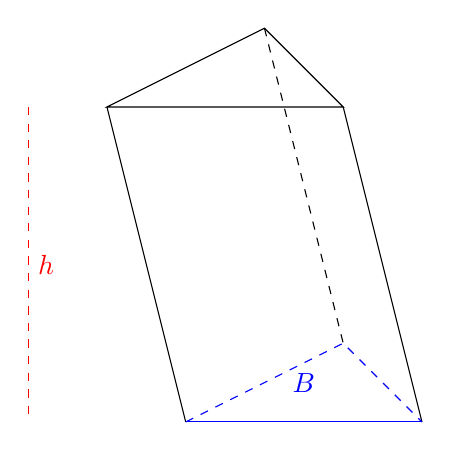
\begin{tikzpicture}
   \draw(0,4) -- (2,5) -- (3,4) --cycle (3,4) -- (4,0) (1,0) -- (0,4);
   \draw[blue] (1,0) -- (4,0);
   \draw[dashed] (2,5) -- (3,1);
   \draw[dashed,blue] (1,0) -- (3,1) -- (4,0);
   \draw[red,dashed] (-1,4) -- (-1,2)node[right]{$h$} -- (-1,0);
   \draw[blue](2.5,.5)node{$B$};
 \end{tikzpicture}
\end{center}

From Wikipedia, uma pirâmide é um poliedro com uma face poligonal (base) e
demais faces triangulares (faces laterais), as quais tem exatamente um ponto em
comum (vértice).
Se $B$ é a área da base e $h$ é a altura do prisma (distância entre o
vértice e o plano da base) o volume do prisma é $V = \frac{1}{3} B \times h$.

\begin{center}
 \begin{tikzpicture}
   \draw (1.5,5) -- (4,0) (1,0) -- (1.5,5);
   \draw[blue] (1,0) -- (4,0);
   \draw[dashed] (1.5,5) -- (3,1);
   \draw[dashed,blue] (1,0) -- (3,1) -- (4,0);
   \draw[red,dashed] (-1,5) -- (-1,2)node[right]{$h$} -- (-1,0);
   \draw[blue](2.5,.5)node{$B$};
 \end{tikzpicture}
\end{center}

\subsection*{Exercício 3}

\begin{enumerate}
\item What is the volume of a a cube of side $a$?
\item We consider the congruent pirâmides of base a face of the cube and vertex
  the center of the cube. How many such pirâmides are there?
\item Deduce the volume of these pirâmides and verify that it is consistent
  with the general expression.
\item Now suppose instead that we have a parallepiped of sides $a,b,c$.
  What is its volume?
\item We consider again the pirâmides of base a face of the parallepiped and
  vertex the center of the parallepiped. Use the general formula to show that
  these pirâmides have the same volume.
\item We consider a pirâmide with base an $n$-gonos for $n \geq 3$.
  Show that if the expression of the volume of a pirâmide is true for tetradros
  ($n=3$) then it is true for any $n$ (consider any diagonal of
  the base).
\end{enumerate}

\subsection*{Exercício 4}

Find the volume of:

\begin{enumerate}
\item A pirâmide of height $h = 8\text{cm}$ and base
  a regular hexagon of side $a=2\text{cm}$?
\item A prisma of height $h=2\text{cm}$ and base a
  rhombus of diagonals $d_1=3\text{cm}$ and $d_2=7\text{cm}$.
\item The pirâmide of base a $P$ and height $h=5\text{cm}$
  where $P$ is a parallelogram of base $b=2\text{cm}$ and altura
  $a=3\text{cm}$.
\item Of the following ``house'' (union of the blue and red poliedros)
  where $h=4\text{m}$, $l=6\text{m}$ and $k = 3\text{m}$.
\begin{center}
 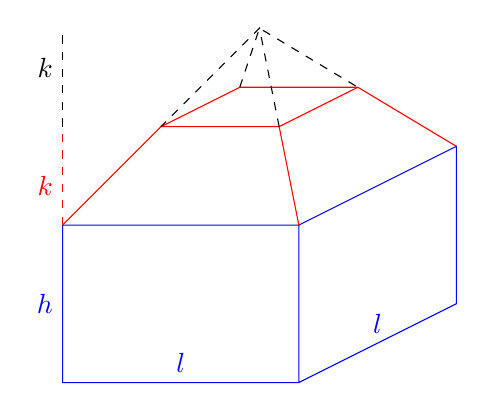
\begin{tikzpicture}
   \draw[color=blue]
   (3,2)-- (3,0)--(1.5,0)node[above]{$l$}-- (0,0)--(0,1)node[left]{$h$}--(0,2)
   -- (3,2)--(5,3)--(5,1)--(4,.5)node[above]{$l$}-- (3,0);
   \draw[color=red] (3,2) -- (2.75,3.25) --  (1.25,3.25) -- (0,2)
   (2.75,3.25) -- (3.75,3.75) -- (5,3)
   (1.25,3.25) -- (2.25,3.75) -- (3.75,3.75);
   \draw[dashed]
   (2.25,3.75) --(2.5,4.5) -- (3.75,3.75)
   (2.75,3.25) -- (2.5,4.5) -- (1.25,3.25)
   ;
   \draw[dashed,color=red]
   (0,2) -- (0,2.5)node[left]{$k$}-- (0,3.25);
   \draw[dashed]
   (0,3.25) -- (0,4)node[left]{$k$}-- (0,4.5);
 \end{tikzpicture}
\end{center}

\end{enumerate}

\subsection*{Exercício 5}

\begin{enumerate}

\item What is the area of a regular tetraedro of side $a$?
\item Viewing the tetraedro as a pirâmide, what are the base and height?
\item Deduce its volume.
\item Recall the area and volume of a cube of side $a$?
\item What is the regular convexo poliedro made by joining
  the centers of a cube of side $a \sqrt{2}$?
\item What is its area?
\item Viewing it has the union of two pirâmides, deduce volume.
\item The regular icosahedron of side $a$ is made of $20$ equilaterales
  triangulos
  of side $a$. What is its area?
\item We use each of these $20$ faces as a base for a pirâmide with vertex
  the center of the icosahedron. We admit that they have height
  $h = \frac{\sqrt{3}}{12} \left(3+\sqrt{5}\right) a$. Deduce the volume
  of the regular icosahedron.
\item A regular dodecahedron
  has area $3 \sqrt{25+10\sqrt{5}}a^2$ and
  volume $\frac{1}{4} \left(15+7\sqrt{5}\right) a^3$.
  Deduce the distance $h$ from the center of one face to the center of the
  dodecahedron.
\end{enumerate}


\section{Cilindros, cones e esferas}

According to Wikipedia, um cilindro é o objeto tridimensional gerado pela
superfície de revolução de um retângulo em torno de um de seus lados.
In the 4º bimestre of the 7ª série do Ensino Fundamental, we saw
a área de um cilindro de altura $h$ e raio $r$ é
%
$$A_{h,r}^{\text{cilindro}} = {2 \pi r^2} + {2\pi r h}$$
%
e o volume do cilindro é
%
$$V_{h,r}^{\text{cilindro}} = A_{r} \times h = \pi r^2 h$$
%
O cone é um sólido geométrico obtido quando se tem uma pirâmide cuja base é um
polígono regular, e o número de lados da base tende ao infinito. From the
formula of the pirâmides we deduce that
%
$$V_{h,r}^{\text{cone}} = \frac{1}{3} \pi r^2 h$$
%
where $r$ is the radius of the base circle and $h$ the height of the cone.
We can prove that its area is given by
%
$$A_{h,r}^{\text{cone}} = \pi r^2 + {\pi r \sqrt{r^2+h^2}}$$
%
Finally, one can prove the following formulas for esferas of radius $r$:
%
$$A_{r}^{\text{esfera}} = 4 \pi r^2$$
%
and
%
$$V_{r}^{\text{esfera}} = \frac{4}{3} \pi r^3$$
%

\subsection*{Exercício 6}

We consider the a cilindro of radius $r$ and height $h=2r$,
a cone of radius $r$ and height $h$ and uma esfera of radius $r$.
Compare their volume and areas.

\subsection*{Exercício 7}

\begin{enumerate}
\item What is approximate
  area and volume of a football ball (circumference of $70\text{cm}$)?
\item What is the volume of ice scream that we can put inside a cone of height
  $h=12\text{cm}$ and
  radius $r=2\text{cm}$, assuming that cone is filled and the volume of ice
  scream at the top is a semi-ball of radius $r$.
\item A cylindric recipient of diameter $10\text{cm}$ and height $3\text{cm}$
  contains some water. We put balls of $1\text{cm}$ of diameters inside the
  recipient and it overflows after putting the $17$-th ball. Deduce the
  approximate volume of water that was present in the recipient.
\end{enumerate}

\section{Solução do Exercícios}

\subsection*{Exercício 1}

\begin{enumerate}
\item The ponto at the center of a classroom and the plano containing the room.
\item The plano containing the blackboard and one ponto drawn on it.
\item The plano containing the top surface of a table and a the reta containing
  a pencil put on it.
\item The plano containing the floor of the classroom and the
  reta containing the intersection of the ceiling and a wall of the room.
\item The reta passing by the center of the top surface of
  a standard rectangular table and the reta containing one leg of the table.
\item The planos containing the floor and ceiling of a classroom.
\item The planos containing the floor and a wall of a classroom.

\end{enumerate}

\subsection*{Exercício 2}

\begin{enumerate}
\item Three pontos that do not belong to a same reta.
\item Yes, using two parallel or concorrentes retas:
  there is only one plano containing them.
\item Yes, if the ponto does not belong to the reta: there is only one plano
  containing them.
\item Una reta (two retas coincidentes), um ponto (e.g. two orthogonal retas),
  or the empty set (e.g. two parallel retas).
\item Una reta (reta included in the plano), um punto
  (e.g. reta orthogonal to um plano) or the empty set (e.g. reta parallel
  but not included in a plano).
\item  Um plano (e.g. two planos coincidentes) or the empty set
  (two parallel planos not coincidentes) or uma reta (two secantes planos).
\end{enumerate}

\subsection*{Exercício 3}

\begin{enumerate}
\item $a^3$
\item There are $6$ such pirâmides (one for each face of the cube).
\item Since these pirâmides are congruent, the volume is
  $\frac{a^3}{6}$. These pirâmides have height $\frac{a}{2}$
  and base a square of area $a^2$ so the general formula gives the same result
  $\frac{1}{3} \times a^2 \times \frac{a}{2} = \frac{a^3}{6}$.
\item $abc$
\item Two of these pirâmides have height $\frac{a}{2}$ and a base a rectangle of
  sides $b,c$ so they have the same volume
  $\frac{1}{3} \times {bc} \times \frac{a}{2} = \frac{abc}{6}$. By symmetry,
  we find the same volume for the 4 other pirâmides.
\item If the base $B$ is an $n$-gono for $n \geq 4$, we can pick a diagonal and
  split the base into two poligonos $B_1, B_2$
  with respectively $p,q < n$ sides, such that $p+q = n$.
  This also gives a partition of the pirâmide into two pirâmide of bases
  $B_1, B_2$ and same vertex and same height $h$.
  By assumption, their volumes are respectively
  $\frac{1}{3} \times {\mathscr{A}(B_1)} \times h$ and
  $\frac{1}{3} \times {\mathscr{A}(B_2)} \times h$ so the initial pirâmide has volume
  $\frac{1}{3} \times {\left({\mathscr{A}(B_1)} + {\mathscr{A}(B_2)}\right)}
  \times h = \frac{1}{3} \times {\mathscr{A}(B)} \times h$.
\end{enumerate}

\subsection*{Exercício 4}
\begin{enumerate}
\item The base is made of $6$ equilateros triangulos of side $a$ so
  has area $\frac{\sqrt{3}}{4}a^2 = 3 \text{cm}^2$. Hence the
  volume of the pirâmide is $\frac{1}{3} \times 3 \times 8 = 8\text{cm}^3$
\item $h \frac{d_1 d_2}{2} = 21 \text{cm}^3$.
\item $P$ has area $ab=6\text{cm}^2$ so the pirâmide has
  volume $\frac{1}{3} h ab = 10\text{cm}^3$.
\item The volume of the blue part is $hl^2 = 144\text{m}^3$.
  The volume of the red part is
  $\left(\frac{1}{3} \times 2k \times l^2\right) -
  \left(\frac{1}{3} \times k \times \left(\frac{l}{2}\right)^2\right) =
  \frac{7}{12} k l^2 = 63 \text{m}^3$. This gives a total
  of $63+144=207\text{m}^3$.

\end{enumerate}

\subsection*{Exercício 5}

\begin{enumerate}
\item The height of a equilaterales triangles of side $a$ is given by
  $\sqrt{a^2 - \left(\frac{a}{2}\right)^2} = \frac{\sqrt{3}}{2} a$.
  So its area is is $\frac{1}{2} \times {\frac{\sqrt{3}}{2} a} \times a =
  \frac{\sqrt{3}}{4}a^2$. Since the regular tetraedro has $4$ faces,
  its area is $\sqrt{3} a^2$.
\item This is a pirâmide of base one equilaterales triangle of side $a$ and
  height joining the center of this triangle to the remaining vertex, that is
  $\sqrt{a^2 - \left(\frac{2}{3} \times \frac{\sqrt{3}}{2} a\right)^2} =
  \sqrt{\frac{2}{3}} a$
\item $\frac{1}{3} \times \sqrt{\frac{2}{3}} a \times \frac{\sqrt{3}}{4}a^2 =
  \frac{\sqrt{2}}{12} a^3$.
\item $6a^2$ and $a^3$
\item It is a regular octaedro of side
  $\sqrt{\left(\frac{a \sqrt{2}}{2}\right)^2 + \left(\frac{a \sqrt{2}}{2}\right)^2} = \sqrt{2 \frac{a^2}{2}} = a$.
\item Each face is a equilateralo
  triangulo of side $a$ so as seen above its area is
  $\frac{\sqrt{3}}{4} a^2$. Since the octaedro has $8$ faces, the total
  area is $2 \sqrt{3} a^2$.
\item We consider the centers $A,B$ of two opposite faces of the cube. The
  other centers form a square $C$ of side $a$. Using $C$ as a base and
  the points $A,B$ as vertices we obtain two congruent pirâmides of height
  $\frac{a \sqrt{2}}{2}$ forming a
  partition of the regular octaedro. Hence the volume is
  $2 \times \frac{1}{3} \times a^2 \times \frac{a \sqrt{2}}{2} = \frac{ \sqrt{2} }{3}a^3$.
\item $20 \times \frac{\sqrt{3}}{4}a^2 = 5\sqrt{3}a^2$
\item $20 \times \frac{1}{3} \times
  \left(\frac{\sqrt{3}}{12} \left(3+\sqrt{5}\right) a\right) \times
  \frac{\sqrt{3}}{4}a^2 = \frac{5 \left(3+\sqrt{5}\right)}{12} a^3$
\item
  $h = 3 \frac{\frac{1}{4} \left(15+7\sqrt{5}\right) a^3}{3 \sqrt{25+10\sqrt{5}}a^2}$.
  After simplification, we can obtain that
  $h^2 = \frac{21\sqrt{5} + 47}{16\sqrt{5}+40} a^2$.
  Then multiplying the numerator and denominator by  $16\sqrt{5}-40$
  we find $h^2 = \frac{11 \sqrt{5} + 25}{40} a^2$ that is
  $h = \frac{1}{2} \sqrt{\frac{11}{10} \sqrt{5} + \frac{5}{2}} a$.

\end{enumerate}

\subsection*{Exercício 6}

The volumes are $V^{\text{cone}} = \frac{2}{3} \pi r^3$,
$V^{\text{esfera}} = \frac{4}{3} \pi r^3$ and
$V^{\text{cilindro}} = 2 \pi r^3$. We note the nice
relations $V^{\text{esfera}} = 2V^{\text{cone}}$ and
$V^{\text{cilindro}} = 3 V^{\text{cone}}$.
The areas are $A^{\text{cone}} = {(1+\sqrt{5})} \pi r^2 <
A^{\text{esfera}} = 4 \pi r^2 <
A^{\text{cilindro}} = 6 \pi r^2$.

\subsection*{Exercício 7}
\begin{enumerate}
\item The radius is $r=\frac{35}{\pi} \text{cm}$.
  So the area is $4 \pi r^2 = \frac{4900}{\pi} \text{cm}^2
  \approx 0.16 \text{m}^2$
  and the volume $\frac{4}{3} \pi r^3 =
  \frac{171500}{3 \pi^2} \text{cm}^3 \approx 5.8 \text{L}$
\item  ${\frac{4}{6} \pi r^3} + {\frac{1}{3} \pi r^2 h} =
  \frac{160\pi}{3} \approx 168 \text{mL}$.
\item The volume added after putting $n$ balls is
  $n \frac{4}{3} \pi \left(\frac{1}{2}\right)^3 = n \frac{\pi}{6} \text{cm}^3$.
  The volume of the recipient is $3 \times \pi \left(\frac{10}{2}\right)^2 =
  75\pi \text{cm}^3$.
  Hence the initial volume of water inside the recipient was between
  $75\pi - 17\frac{\pi}{6} = \frac{433}{6} \pi \text{cm}^2$ and
  $75\pi - 16\frac{\pi}{6} = \frac{217}{3} \pi \text{cm}^2$ that is
  approximately $227\text{mL}$.
\end{enumerate}
